\documentclass[12pt, letterpaper]{article}  % change to >11 pt if you like, and change article with report
\usepackage[letterpaper, top=3.71cm, bottom=3.20cm, left=2.86cm, right=2.86cm]{geometry}
\usepackage[utf8]{inputenc}
\usepackage{natbib}
\usepackage{graphicx}
\usepackage{color}
\usepackage{subfig}
\usepackage{float}
\usepackage{hyperref}
\usepackage{url}
\usepackage{listings}
%\usepackage{pythontex}
\definecolor{bg}{gray}{0.95}
\usepackage{minted}

\title{\vspace{-2cm}\textbf{Human Language Technologies project report}}
\author{\textbf{\small{\textit{Dalla Noce Niko, Ristori Alessandro}}} \\ % put your full name here
        \small{Master Degree in Computer science.}\\ \small{{n.dallanoce@studenti.unipi.it, a.ristori5@studenti.unipi.it}.} \\  % put your Master Degree here
        \small{Human Language Technologies, Academic Year: 2020/2021} \\
        \small{Date: 10/05/2021} \\
       \textbf{\small{\url{https://github.com/nikodallanoce/HLT}}}
}

\renewcommand\refname{} %remove this line to automatically show the bibliography header

\begin{document}

\nocite{*}  % comment this line to list only the articles you really cite
\date{}
\maketitle
\begin{center}
    
\includegraphics[width=0.2\textwidth]{images/unipi.png}\\
    \vspace{0.5cm}
\end{center}
\begin{abstract}
The report starts with a long, but needed introduction to the main concepts that we've seen during the course of our work and it shows what was our purpose and how we reached it. Then it shows the results obtained by the models we tried giving at the same time the reasons of their performances. The report concludes with our final considerations on what and how we could have done more.
\end{abstract}
\newpage
\tableofcontents
\newpage
\listoffigures
\section{Introduction}
Before we dive into our work, we talk briefly about our task and introduce the key concepts and models that we used during our project.
\subsection{Task}
The purpose of our task was to understand and implements NMT models and do a comparison between them and state-of-art models, for doing so we had to build an encoder-decoder from scratch and then we exploited the transformers available on Hugginface.com \cite{huggingface_co} to improve the performance of our model. The best one was then pushed even further by feeding it more records during training and letting it run for more epochs in hope to achieve a better revisited BLEU score \cite{goyal2021flores}. As for the datasets we used the english-italian one from manythings.com\cite{anki_dataset} and the en-it europarl \cite{koehn2005europarl}, which, combined, resulted in more than 2 milion records, not enough to reach the perfomances of state-of-art models, but still useful to achieve nice results.
\vspace{3mm}

Over the next subsections, we'll talk about NMT and the models used for our work and their architecture, to give a better insight on their peculiarities and how we tried to exploit them.
\subsection{Neural Machine Translation}\label{subsec:NMT}
Neural Machine Translation, or simply NMT, is an approach to translate sentences from one language into another one (e.g.: from english to italian) by using a single neural network whose architecture is based on the encoder-decoder paradigm.
In its easiest form the network is composed by two RNNs (LSTMs or GRUs), one for the encoder and one for the decoder, that are trained jointly, in an end-to-end fashion, for maximizing the translation performance; such model composed of two RNNs has a very straight forward way of working:
\begin{itemize}
    \item The \textbf{encoder} receives one sentence from the source language and produces an encoding from it, such encoding will provide the fist hidden state of the decoder;
    \item The \textbf{decoder} receives the encoding produced by the encoder and builds the sentence in the target language one word at time conditioned on the encoding.
\end{itemize}
\begin{figure}[H]%
    \centering
    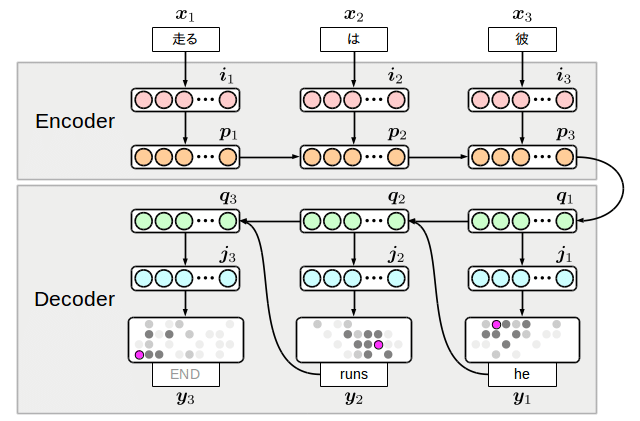
\includegraphics[width=0.65\linewidth]{images/seq2seq.png}
    \caption{Standard NMT model}
    \label{fig:NMT_model}
\end{figure}
This extremely simple model beat all the previous paradigms by a large margin providing more fluent and precise context-wise translations and its training was even easier since both parts, encoder and decoder, are trained together giving less headaches on optmizing every single sub-module.
\subsection{Transformer}\label{subsec:transformer_model}
In \ref{subsec:NMT} we've talked about a very simple model composed by two RNNs, one for the encoder and one for the decoder, but a more powerful and complex architecture was introduced by Vaswani et al. \cite{vaswani2017attention} called transformer that disposes of any recurrent or convolutional layer and relies solely on attention. The transformer still follows the encoder-decoder paradigm, but both parts are now composed by multiple layers and sub-layers:
\begin{itemize}
    \item \textbf{Encoder}\\
    The encoder is composed of a stack of N identical layers and each layer has two sub-layers. The first is a multi-head self-attention mechanism, and the second is a position-wise fully connected feed-forward network. Each of the two sub-layers is followed by layer normalization. All sub-layers in the model, as well as the embedding layer, produce outputs of the same dimension.
    \item \textbf{Decoder}\\
    The decoder is also composed of a stack of N identical layers. The decoder inserts a third sub-layer, which performs multi-head attention over the output of the encoder stack. Similar to the encoder, each of the sub-layers is followed by layer normalization. We also modify the self-attention sub-layer in the decoder stack to prevent positions from attending to subsequent positions. This masking, combined with fact that the output embeddings are offset by one position, ensures that the predictions for position i can depend only on the known outputs at positions less than i.
\end{itemize}
\begin{figure}[H]%
    \centering
    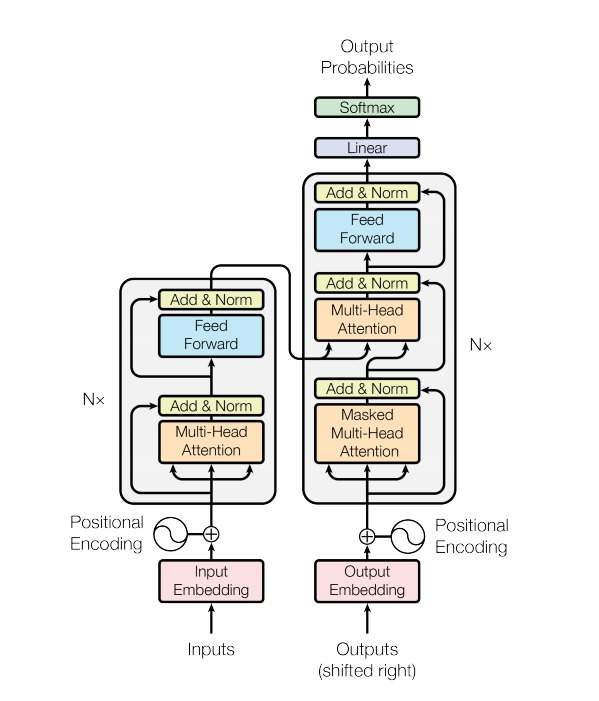
\includegraphics[width=0.68\linewidth]{images/transformer.png}
    \caption{Transformer model}
    \label{fig:transformer}
\end{figure}
\subsubsection{Self and multi-head attention}
The particular attention used by Vaswani et al. \cite{vaswani2017attention} is called "Scaled Dot-Product Attention" (Figure \ref{fig:transformer_attention} on the right). The input consists of queries and keys of dimension $dk$, and values of dimension $dv$. We compute the dot products of the query with all keys, divide each by $\sqrt{dk}$, and apply a softmax function to obtain the weights on the values.
\begin{figure}[H]%
    \centering
    \subfigure[Multi-Head Attention]{{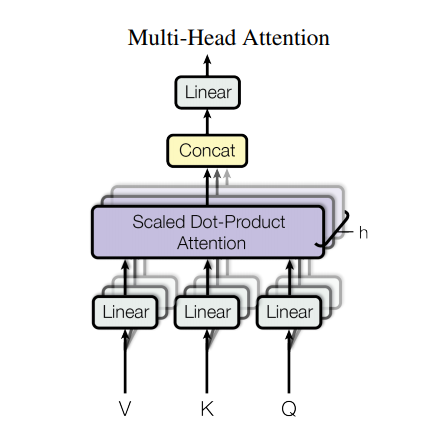
\includegraphics[width=0.4\linewidth]{images/multi_head_attention.png}}}%
    \subfigure[Scaled Dot-Product Attention]{{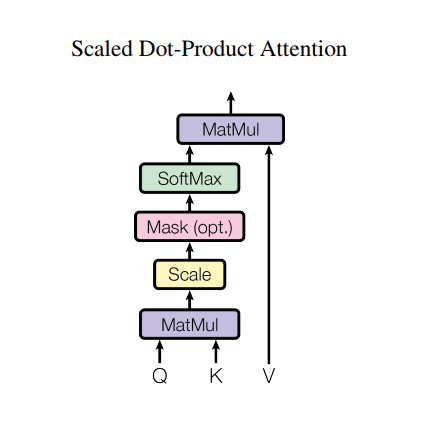
\includegraphics[width=0.4\linewidth]{images/self_attention.png}}}%
    \caption{On the left the multi-head attention is shown composed by multiple heads, on the right the single Scaled Dot-Product Attention mechanism.}
    \label{fig:transformer_attention}%
\end{figure}
The attention function is computed on a set of queries simultaneously, packed together into a matrix Q. The keys and values are also packed together into matrices K and V . We compute the matrix of outputs as:
\begin{large}
$$Attention(Q, K, V ) = softmax(\frac{QK^T}{\sqrt{dk}})V$$
\end{large}
Instead of performing a single attention function with keys, values and queries whose dimension is based on the model dimension, it is beneficial to linearly project the queries, keys and values h times with different, learned linear projections to dk, dk and dv dimensions, respectively. On each of these projected versions of queries, keys and values we then perform the attention function in parallel, yielding $dv$-dimensional output values. These are concatenated and once again projected, resulting in the final values, as depicted in Figure \ref{fig:transformer_attention} on the left.
Multi-head attention allows the model to jointly attend to information from different representation subspaces at different positions.
\begin{large}
$$MultiHead(Q, K, V ) = Concat(head_{1}, ..., head_{h})W^O$$
\begin{center}where\end{center}
$$head_{i} = Attention(QW^Q_{i}, KW^K_{i}, VW^V_{i})$$
\end{large}
If we call h as the number of parallel attention layers, or heads, for each of these we use $dk=dv=dmodel/h$ as dimension. Due to the reduced dimension of each head, the total computational cost is similar to that of single-head attention with full dimensionality.
\subsection{BERT and DistilBERT}\label{subsec:bert}
BERT (Bidirectional Encoder Representations from Transformers) is a multi-layer bidirectional Transformer encoder introduced by Drevlin et al. \cite{devlin2018bert} and  based on the original transformer implementation described in Vaswani et al. \cite{vaswani2017attention}.
\begin{figure}[H]%
    \centering
    \subfigure[BERT single layer]{{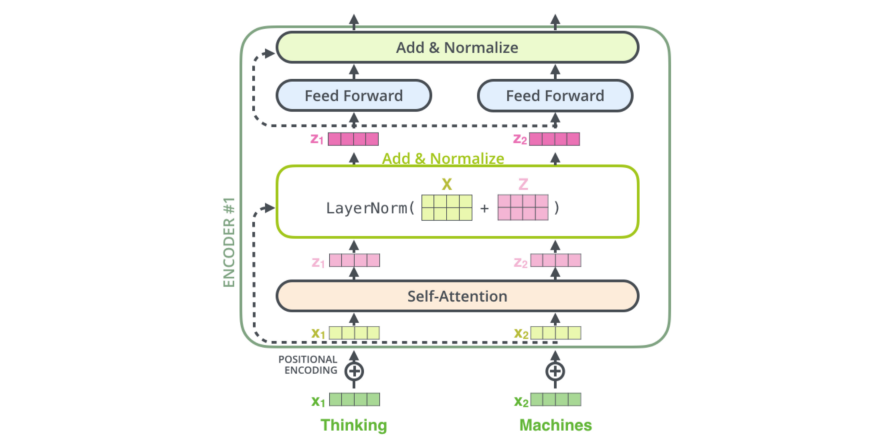
\includegraphics[width=0.50\linewidth]{images/bert_layer.png}}}%
    \subfigure[BERT stacked layers]{{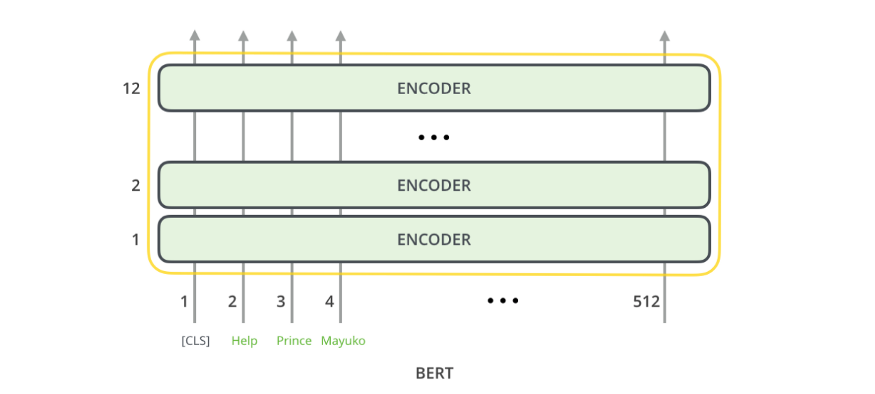
\includegraphics[width=0.50\linewidth]{images/bert_layers.png}}}%
    \caption{BERT architecture}
    \label{fig:bert}%
\end{figure}
BERT is conceptually simple and empirically powerful and that's why we decided to use it in our project, even though it's not aimed at NMT (its purpose are masked language tasks) it still provides great performances for our work, but BERT is extremely big even in his base form (it contains twelve layers, as many as a standar transformer) so it isn't the most cost-efficient model for our task, so for this reason we opted to use its distilled\footnote{Knowledge distillation is a compression technique in which a compact model - the student - is trained to reproduce the behaviour of a larger model - the teacher - or an ensemble of models.} version, called DistilBERT \cite{sanh2019distilbert}.
\vspace{3mm}

DistilBERT is a small, fast, cheap and light Transformer model trained by distilling BERT. It has 40\% less parameters than BERT, runs 60\% faster while preserving over 95\% of BERT’s performances as measured on the GLUE language understanding benchmark \cite{wang2018glue}. For those reasons, DistilBERT was chosen instead of BERT since we didn't have very powerful machines in our hands.

\subsection{RoBERTa}
Roberta is a transformer encoder with the same architecture as BERT, described in \ref{subsec:bert}, developed by Facebook AI. As written by Liu et al. \cite{liu2019roberta}, the team found that BERT was significantly undertrained, and can match or exceed the performance of every model published after it. They have just modified BERT key hyperparameters, removing the next-sentence pre-training objective and training with much larger mini-batches and learning rates. In 2019, when Facebook AI wrote the article, their best model achieved state-of-the-art results on GLUE \cite{wang2018glue}, RACE and SQuAD.
\subsection{T5v11}
A Google research team published the paper by Raffel et al. \cite{raffel2019exploring}, introducing a novel “Text-to-Text Transfer Transformer” (T5) transformer model which can convert any language problem into a text-to-text format.
\begin{figure}[H]
    \centering
    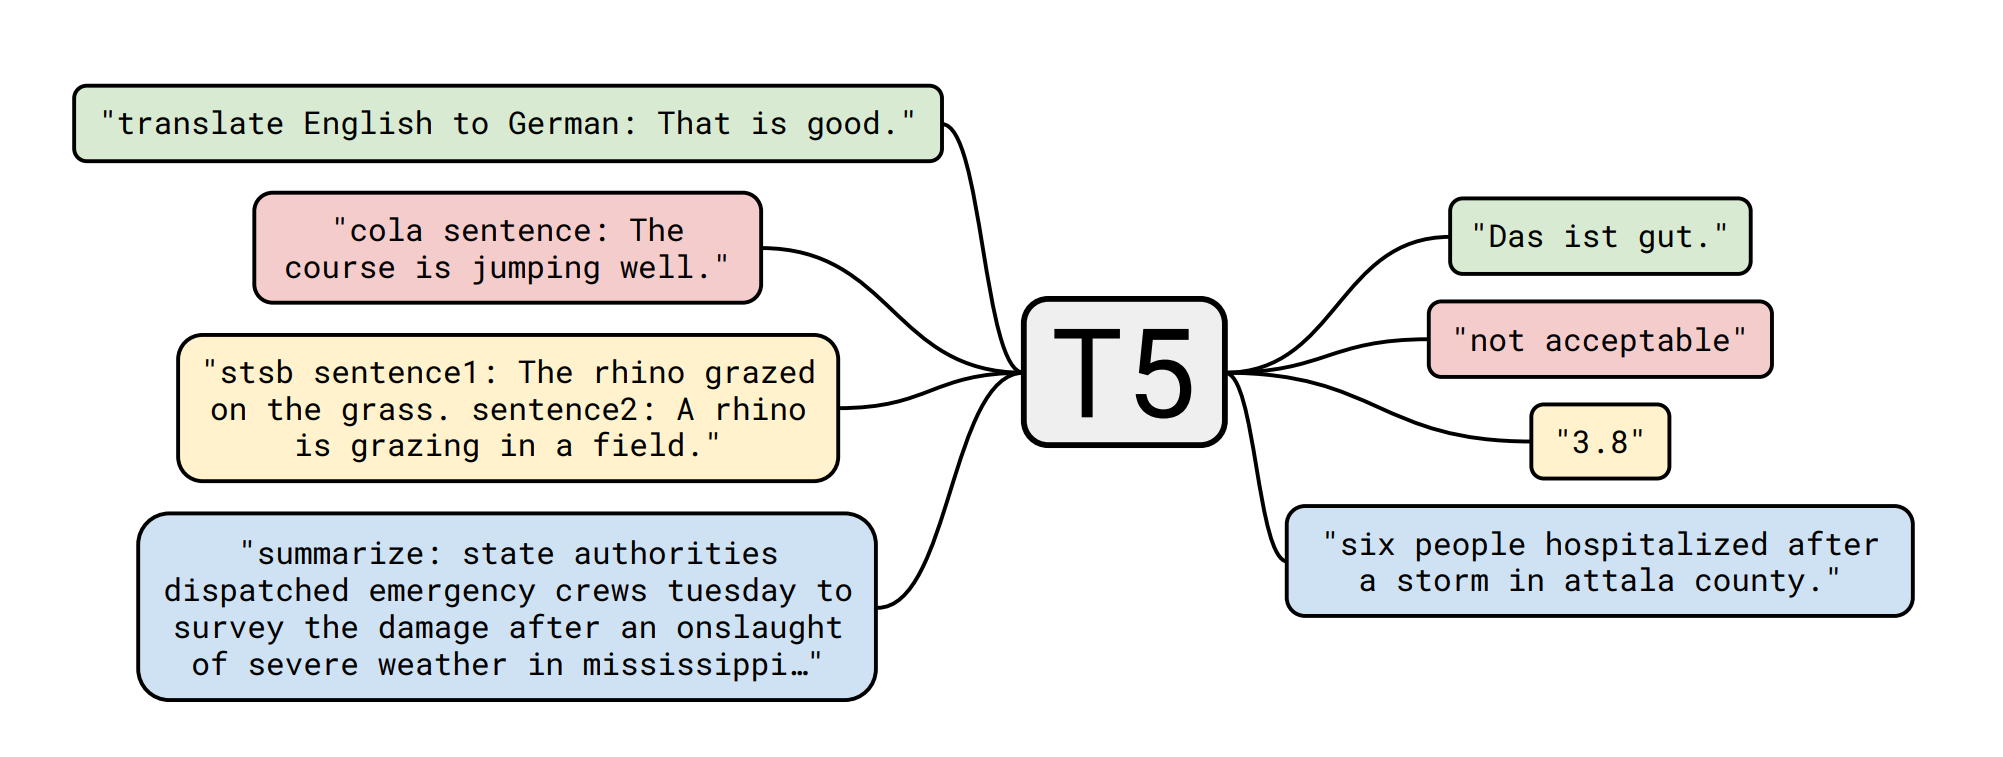
\includegraphics[width = .7\linewidth]{images/google_T5.png}
    \caption{Google T5 model.}
    \label{fig:google_t5}
\end{figure}
The idea behind T5 was to exploit the potential of transfer learning, where a model is first pre-trained on a data-rich task before being fine-tuned on a downstream task, emerging as a powerful technique in natural language processing (NLP). The proposed model is essentially a Encoder-Decoder Transformer with some architectural changes (like applying Layer Normalization before a sub block and then adding the initial input to the sub-block output; also known as pre-norm).
\vspace{3mm}

The model configuration is similar to BERT base and we decided to use the more polished version, T5v11, since it had some improvements:
\begin{itemize}
    \item GEGLU activation in the feed-forward hidden layer, rather than ReLU.
    \item Dropout was turned off in pre-training (quality win). Dropout should be re-enabled during fine-tuning (which we did).
    \item Pre-trained on C4 only without mixing in the downstream tasks.
    \item No parameter sharing between the embedding and classifier layer.
\end{itemize}
Between all the transformers models we considered for the project, T5 was the only one aimed at an NMT task, so we expected it to give us better performances than the previous models we've shown.
\section{Datasets and benchmark}\label{sec:dataset}
Before talking about the workflow and the results, we thought it was necessary to explain the datasets we used and how we preprocessed them. At the beginning we first tried to use the  europarl en-it corpus, however we've found ourselves overwhelmed by the dataset's huge size, moreover it was filled with extremely long sentences, so the training phase of our model was extremely time-consuming, even on Colab TPUs. As a consequence, we tried using only an half of the original dataset but the model did not translate well. To overcome those difficulties,  we decided to adopt a second dataset, the en-it anki corpus which contains way less records than the first one (with more sentences used in a normal conversation), but enough to build a simple and well behaved NMT model.
\subsection{ANKI en-it dataset}
The anki corpus from \cite{anki_dataset} to work on was the english-italian one which contained 352040 records at the time of our download and then we preprocessed and divided it in our development (training and validation) and test sets.
\subsubsection{Preprocessing the anki corpus}
The corpus was, luckily, without any issue, we just had to take away the copyrights from each single sentence pair, which was done by a simple python method. Moreover we had two versions of the corpus, one with no copyright and one without, the method takes care of this case too.
\begin{comment}
\begin{minted}{python}
def create_dataset_anki(name: str, preprocessed: bool = False):
    with open(name, encoding="UTF-8") as datafile:
        src_set = list()
        dst_set = list()
        for sentence in datafile:
            sentence = sentence.split("\t")
            src_set.append(sentence[0])
            if preprocessed:
                dst_set.append(sentence[1].split("\n")[0])
            else:
                dst_set.append(sentence[1])

    return src_set, dst_set
\end{minted}
\end{comment}
The method returns two lists, one for the english sentences and one for the italian ones, we then tokenized both the lists and we proceeded with the creation of our training, validation and test sets with the (0.8, 0.1, 0.1) split.
At this point the training set is divided in batches and is ready to be fed to the model.
\subsection{EuroParl en-it dataset}
Since the anki dataset consists of very simple sentences, we thought that it would be better for our model to include some records from the europarl dataset.
\subsubsection{Preprocessing the europarl corpus}
As for the anki dataset, luckily for us the europarl corpus was already largely preprocessed, the main issue was the huge size which meant that the dataset couldn't fit inside the allocated memory on colab, that's why we decided to take only a fifth of the initial corpus (381823 records).
\begin{comment}
\begin{minted}{python}
def create_dataset_euparl(name: str, src: str = "en", dst: str = "it",
                        size: float = 1) -> (list, list):
    with open(name+".{0}".format(src), encoding="UTF-8") as datafile:
        src_set = datafile.readlines()

    with open(name+".{0}".format(dst), encoding="UTF-8") as datafile:
        dst_set = datafile.readlines()

    if size != 1:
        if size > 1 or size < 0:
            raise ValueError("No correct size for the euparl corpus")
        
        datasets_to_shuffle = list((zip(src_set, dst_set)))
        np.random.shuffle(datasets_to_shuffle)
        src_set, dst_set = zip(*datasets_to_shuffle)
        src_set = list(src_set[:int(len(src_set) * size)])
        dst_set = list(dst_set[:int(len(dst_set) * size)])
        
    return src_set, dst_set
\end{minted}
\end{comment}
\subsection{Merging the datasets}
We merged the two datasets in hope to have a better performance on our models, so we have 733863 records to be splitted into training, validation and test sets.
\begin{minted}{python}
def merge_datasets(first_dataset, second_dataset) -> (list, list):
    first_src, first_dst = first_dataset
    second_src, second_dst = second_dataset
    src_set = first_src + second_src
    dst_set = first_dst + second_dst
    return src_set, dst_set
\end{minted}
The split was (0.8, 0.1, 0.1) resulting in the following size for our sets:
\begin{itemize}
    \item Training set size: 587090.
    \item Validation set size: 73386.
    \item Test set size: 73387.
\end{itemize}
The sets are then splitted into batches to improve the training done by the keras fit method.

\subsection{Benchmark}
We found a recently developed benchmark based on SacreBLEU for our project which is the flores dataset built by \cite{goyal2021flores}, it was developed by Facebook and it's useful for those languages with not so many resources (italian doesn't have many evaluation datasets around) and for assessing not so huge models, which is perfect for our case.
\vspace{3mm}

The benchmark, as we said before, is based on SacreBLEU( which is an improved version of BLEU that expects detokenized sentence to evaluate a model performances developed by \cite{post2018call}) and comes with a test set composed by 1012 sentences taken from the english wikipedia and translated by humans, so each of our models were evaluated on how they performed on that set.

%\section{Task Workflow}\label{sec:task_workflow}
Our task, and the main requisite of the project, was building a NMT model based on the transformer architecture, moreover we had to insert BERT into our model as an encoder to test its performances.
\subsection{Tokenization}\label{subsec:tokenization}
As first step into oure task, we had to tokenize the datasets seen in section \ref{sec:dataset}, we opted for the BertTokenizer from huggingface.com instead of building one of our own, since it would have been essential for working with BERT later on the project. After loading the tokenizers, one for each language, we proceed with the tokenization of the entire dataset.
\begin{minted}{python}
en_set, it_set = create_dataset_anki("dataset/ita.txt")

# Load the tokenizers and get the number of tokens
tokenizer_en = BertTokenizer.from_pretrained("bert-base-uncased")
tokenizer_it = BertTokenizer.from_pretrained("dbmdz/"
                                             "bert-base-italian-uncased")
v_size_en = tokenizer_en.vocab_size
v_size_it = tokenizer_it.vocab_size

# Tokenize the dataset
tokens_en = tokenizer_en(en_set, add_special_tokens=True,
                         truncation=True, padding="max_length", 
                         return_attention_mask=True, return_tensors="tf",
                         max_length=30).data["input_ids"]
tokens_it = tokenizer_it(it_set, add_special_tokens=True,
                         truncation=True, padding="max_length", 
                         return_attention_mask=True, return_tensors="tf",
                         max_length=30).data["input_ids"]
\end{minted}

By looking at the previous code snippet we have to explain how and what the BERT tokenizer returns from such method.
Beside the input tokens we also got 2 special tokens ‘[CLS]’ and ‘[SEP]’, BERT is designed in such a way that the sentence has to start with the [CLS] token and end with the [SEP] token to separate sentence from sentence. The padding is set to a defined max\_length value which, as its name suggests, specifies the maximum length for all the pattern (so we they only one dimension, useful for training and inference) and it's calculated such that the 95\% of the sentences are fully tokenized.
\vspace{3mm}

The tokenizer returns a tuple containing three tensors, from which we only retrieve the first:
\begin{itemize}
    \item \textbf{input\_ids}\\
    The tokens tensors, which will be used to build our tensorflow dataset.
    \item \textbf{attention\_mask}\\
    As the name says is the mask passed to the attention layer that tells in which positions the layer must attend, is filled with ones where the tokens aren't zero and zeros in any other case.
    \item \textbf{token\_type\_ids}\\
    The final tensor is the one that many tokenizers or transformers don't use (such as distillBERT), it 
\end{itemize}
%For our purpose we opted to think about encoder and decoder as blocks (more specifically as keras.layers.Layer subclasses) which can be of different types. As an example the encoder can be chosen beetween the following (the decoder implements only the first two, since we can't use BERT for that purpose):
%\begin{itemize}
%    \item \textbf{RNN}\\
%    A simple encoder with a bidirectional GRU layer inside.
%    \item \textbf{Transformer}\\
%    The strucute is shown in \ref{fig:transformer}, the user can decide the number of layers and attention-head while setting up the layer.
%    \item \textbf{BERT}\\
%    This encoder layer wraps a BERT model from huggingface.com and builds all the mandatory things for its work.
%\end{itemize}
\section{Workflow}
\subsection{Setup}
\paragraph{Hardware}
Models were being trained in Google Colab using Google TPU v2 \footnote{\url{https://cloud.google.com/tpu}}. It has 64 GB HBM memory and a compute capability of 180 teraflops. In our experiments, TPUs outperform NVidia GPUs available in Colab by running six time faster.
\paragraph{Software}
In order to train transformer models, we used Tensorflow with Keras \cite{keras_io} and the Huggingface \cite{huggingface_co} python library to retrieve pre-trained models.

\subsection{Dataset management}
As a guideline, we trained our models using the entire anki dataset and 20 percent of the Europarl bilingual dataset. In order to train a model for machine translation, the sentences inside the datasets that are written in natural language have to be preprocessed. This phase is called tokenization. Every encoder has its own tokenizer, that is a module that parse words into tokens, that are integers essentially. These two datasets don't fit together into the RAM available in Google Colab, so it was necessary to split them into smaller one in order to apply the tokenizer. After that every tokenization on the small piece of the dataset was completed, we merge the results using Tensorflow Dataset API, in order to build the entire tokenized dataset. This is a mandatory step that allow to train any model using very large dataset. In fact, Tensorflow Dataset swaps data into the secondary memory if the main memory in not enough to contain the entire data. At training time, Tensorflow Dataset loads data into the accelerator (GPU or TPU) memory in batches of equal dimension. 

\subsection{Tokenization}
As announced earlier, any dataset made up of sentences written in natural language has to be tokenized before its usage. The Huggingface library provides a Tokenizer class that can retrieve a pre-trained tokenizer from a wide database and tokenize any sentence you provide. As shown in the example below in code \ref{lst:bert_tokenizer}, we create a dataset with a fixed length of tokens, padded with zeros whether the sentence was shorter than the maximum length or truncated in case it exceed the pre-defined size.
\begin{listing}[H]
\begin{minted}[fontsize=\small, linenos, breaklines]{python}
tok_trg = "dbmdz/bert-base-italian-cased"
tokenizer_target = BertTokenizerFast.from_pretrained(tok_trg) 
tokens_source = tokenizer_source(source_set, truncation=True,                      padding="max_length", return_tensors="tf",                         max_length=sequence_length).data["input_ids"]
\end{minted}
\caption{Example of code to tokenize a piece of dataset using Huggingface Bert Tokenizer.}
\label{lst:bert_tokenizer}
\end{listing}
\section*{References}
%From where you are taking information, where a reader can find details, credits, sources \dots See any paper bibliography to take examples. The items here should be numbered and the number should be used in the text. \textbf{Double check the bibliography}!!! \\ \\
%In particular, always include (with a uniform style): \\

%Authors, Title, Journal/Proceedings/Editor, Volume, Pages, Year (URL if needed) \\ %\\
%E.g.: 
\bibliographystyle{plain}
\vspace{-1cm}\bibliography{references}

\end{document}

